\chapter{Progress Report}
\section{Project Status}
The project is currently in the assembly phase after having successfully completed the concept design and selection phase, detailed design phase, and most of the parts sourcing phase. There are one or two more small items that need to be bought, but the majority of the key components have been sourced and will be arriving on Tuesday 30 July. All laser cut parts have been finished and are ready for assembly, as seen in figure \ref{fig:laser_cut_parts}. The MM workshop will start with my drawings on the week after this report hand in, I expect to start assembly at the end of next week. The lab safety report has been completed and is awaiting signing from the necessary parties before the lab can be used.

\begin{figure}[H]
    \centering
    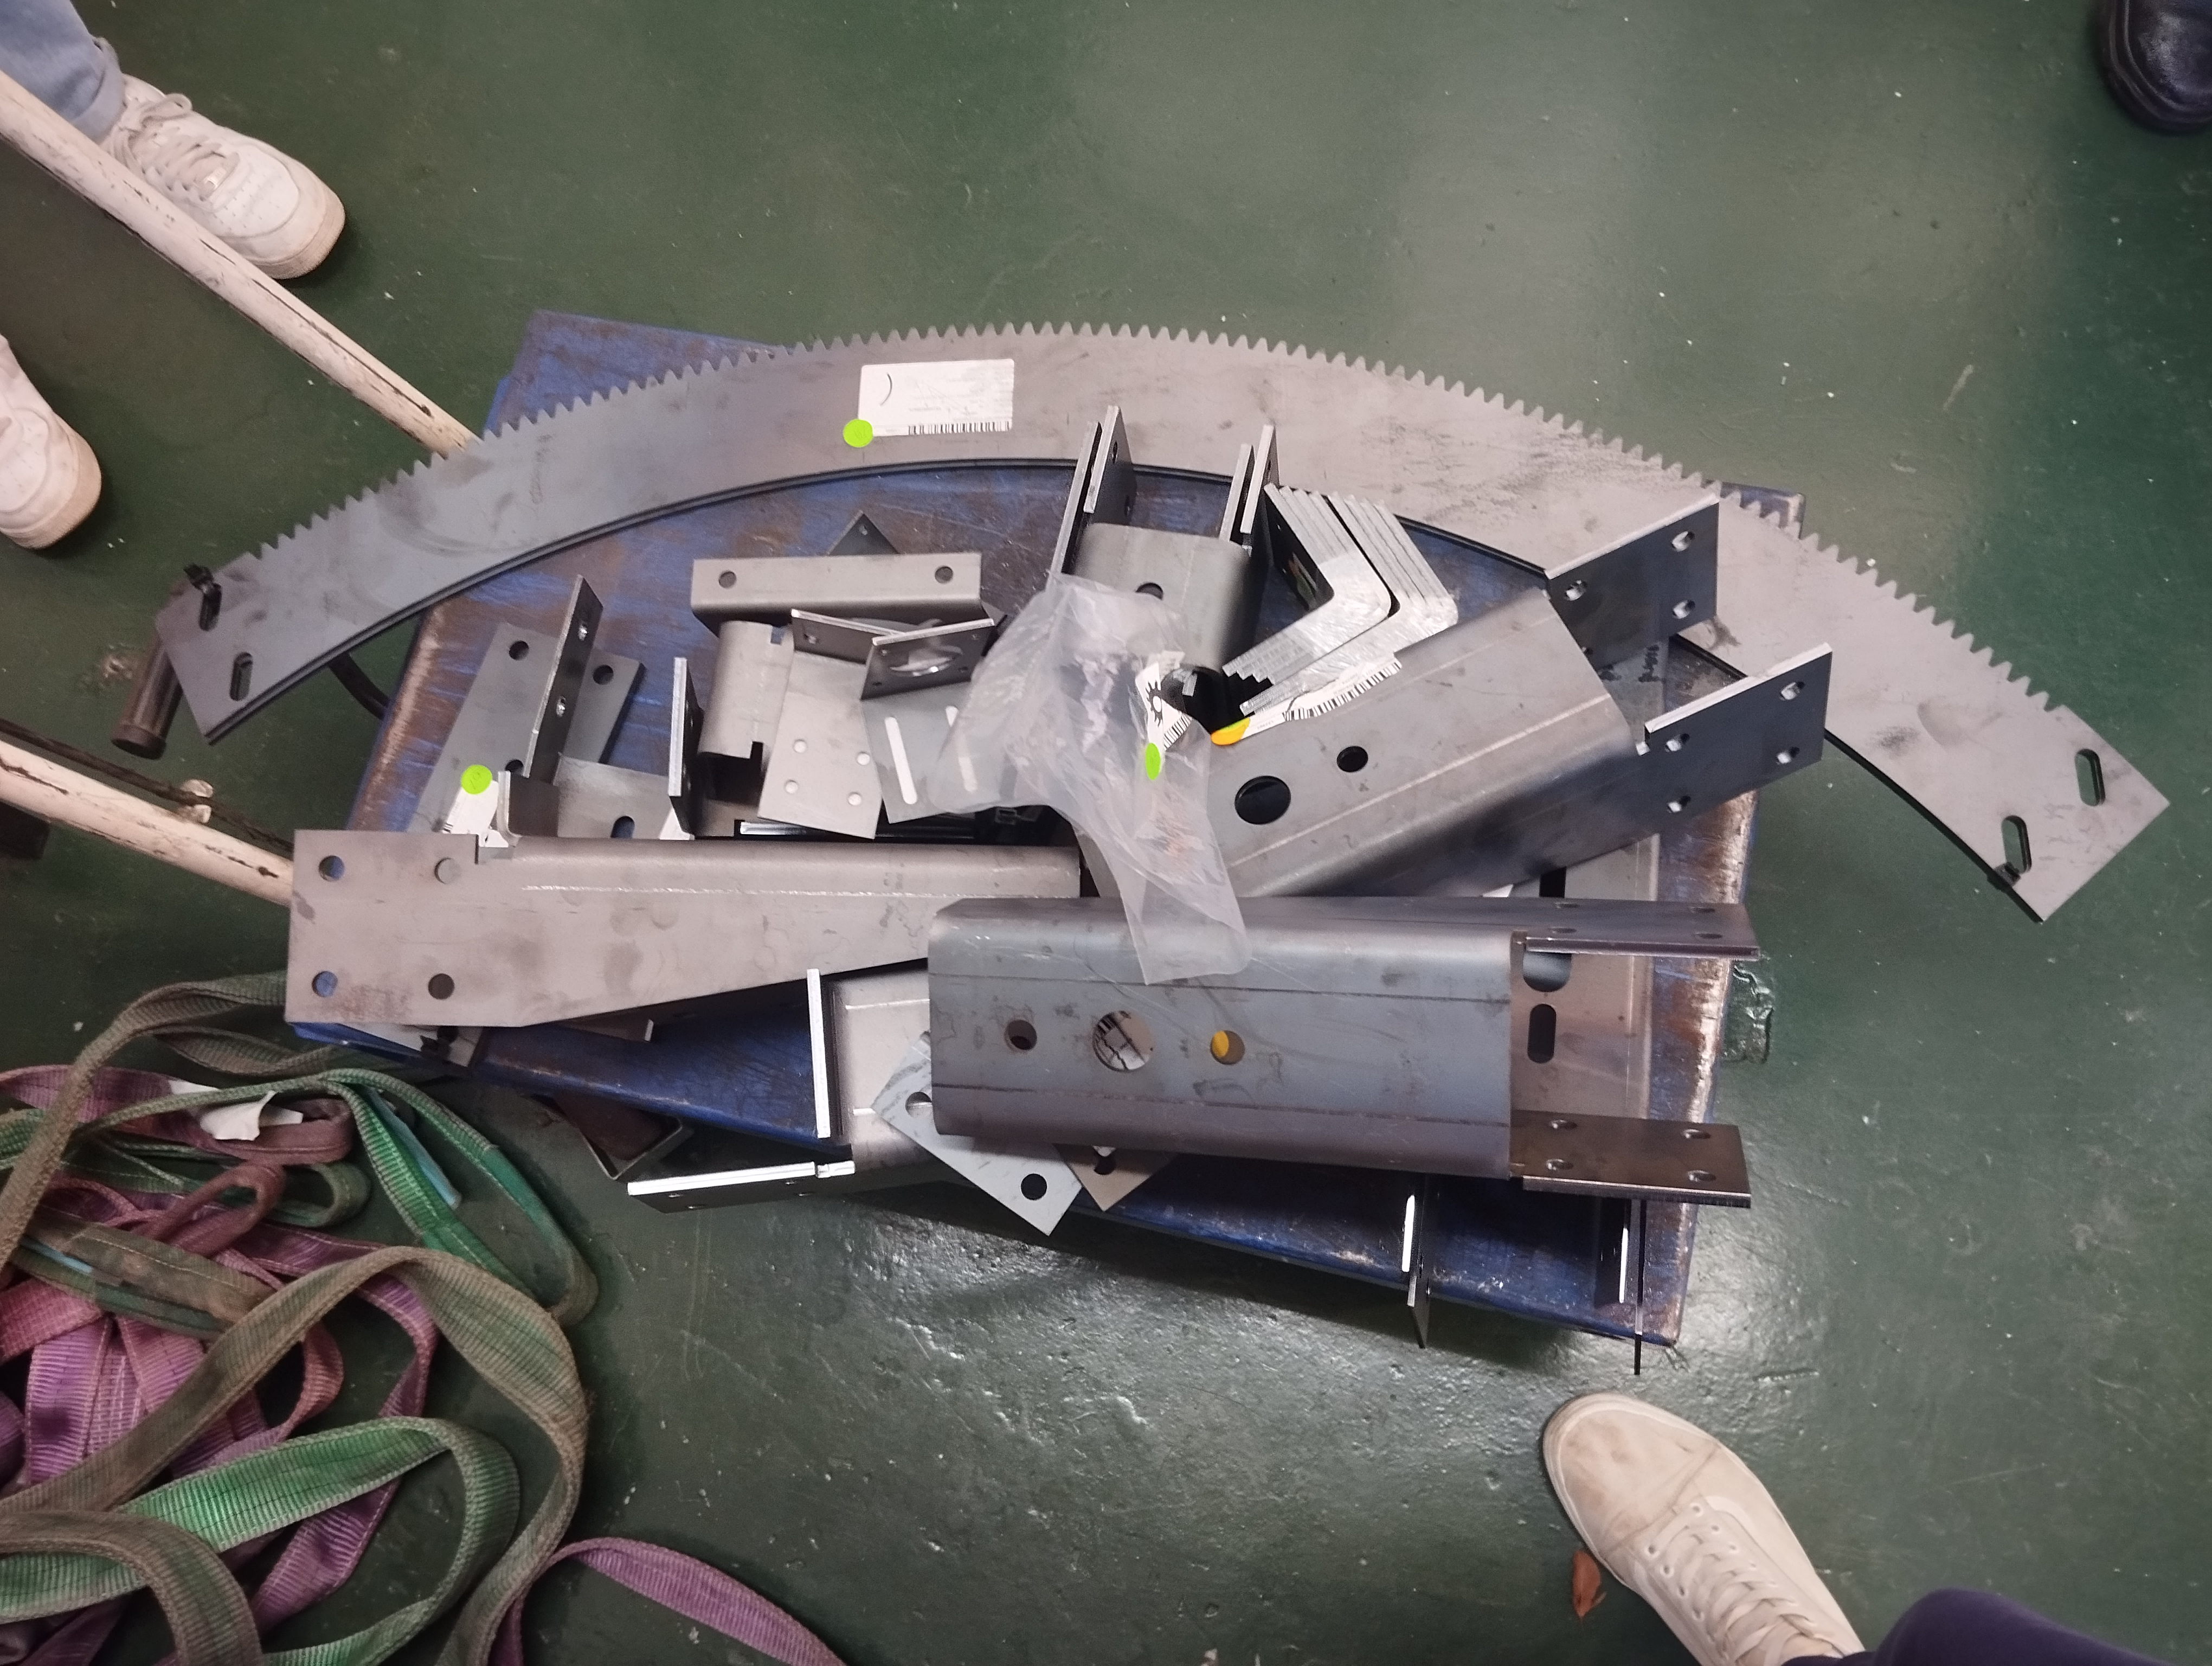
\includegraphics[width=0.75\linewidth]{figs/laser_cut_parts.jpg}
    \caption{Completed Laser Cut Parts}
    \label{fig:laser_cut_parts}
\end{figure}

\section{Planned Revision}
\subsection{Reevaluation of Design Choices}
Design choices made during the initial phases of the project have been periodically reevaluated and altered in order to keep aligned with project goals, design, and stakeholder requirements.
\subsection{Major Revisions}
There have been no major revisions to the project plan thus far, as it has been adhered to as closely as possible. However, I acknowledge the possibility of redesigning certain components after construction begins. Should these changes become necessary, they will be implemented swiftly and effectively to minimize any impact on the project schedule.


\section{Project Schedule}
The project is still on time, although is slightly behind schedule according to the  gantt chart created for the project proposal. The proposed gantt chart is depicted in figure \ref{fig:initial-gantt} and shows that construction was planned to begin midway through June, although I believe that I will be able to complete construction swiftly with enough time to complete the report by the deadline. 

\begin{figure}[ht]
    \centering
    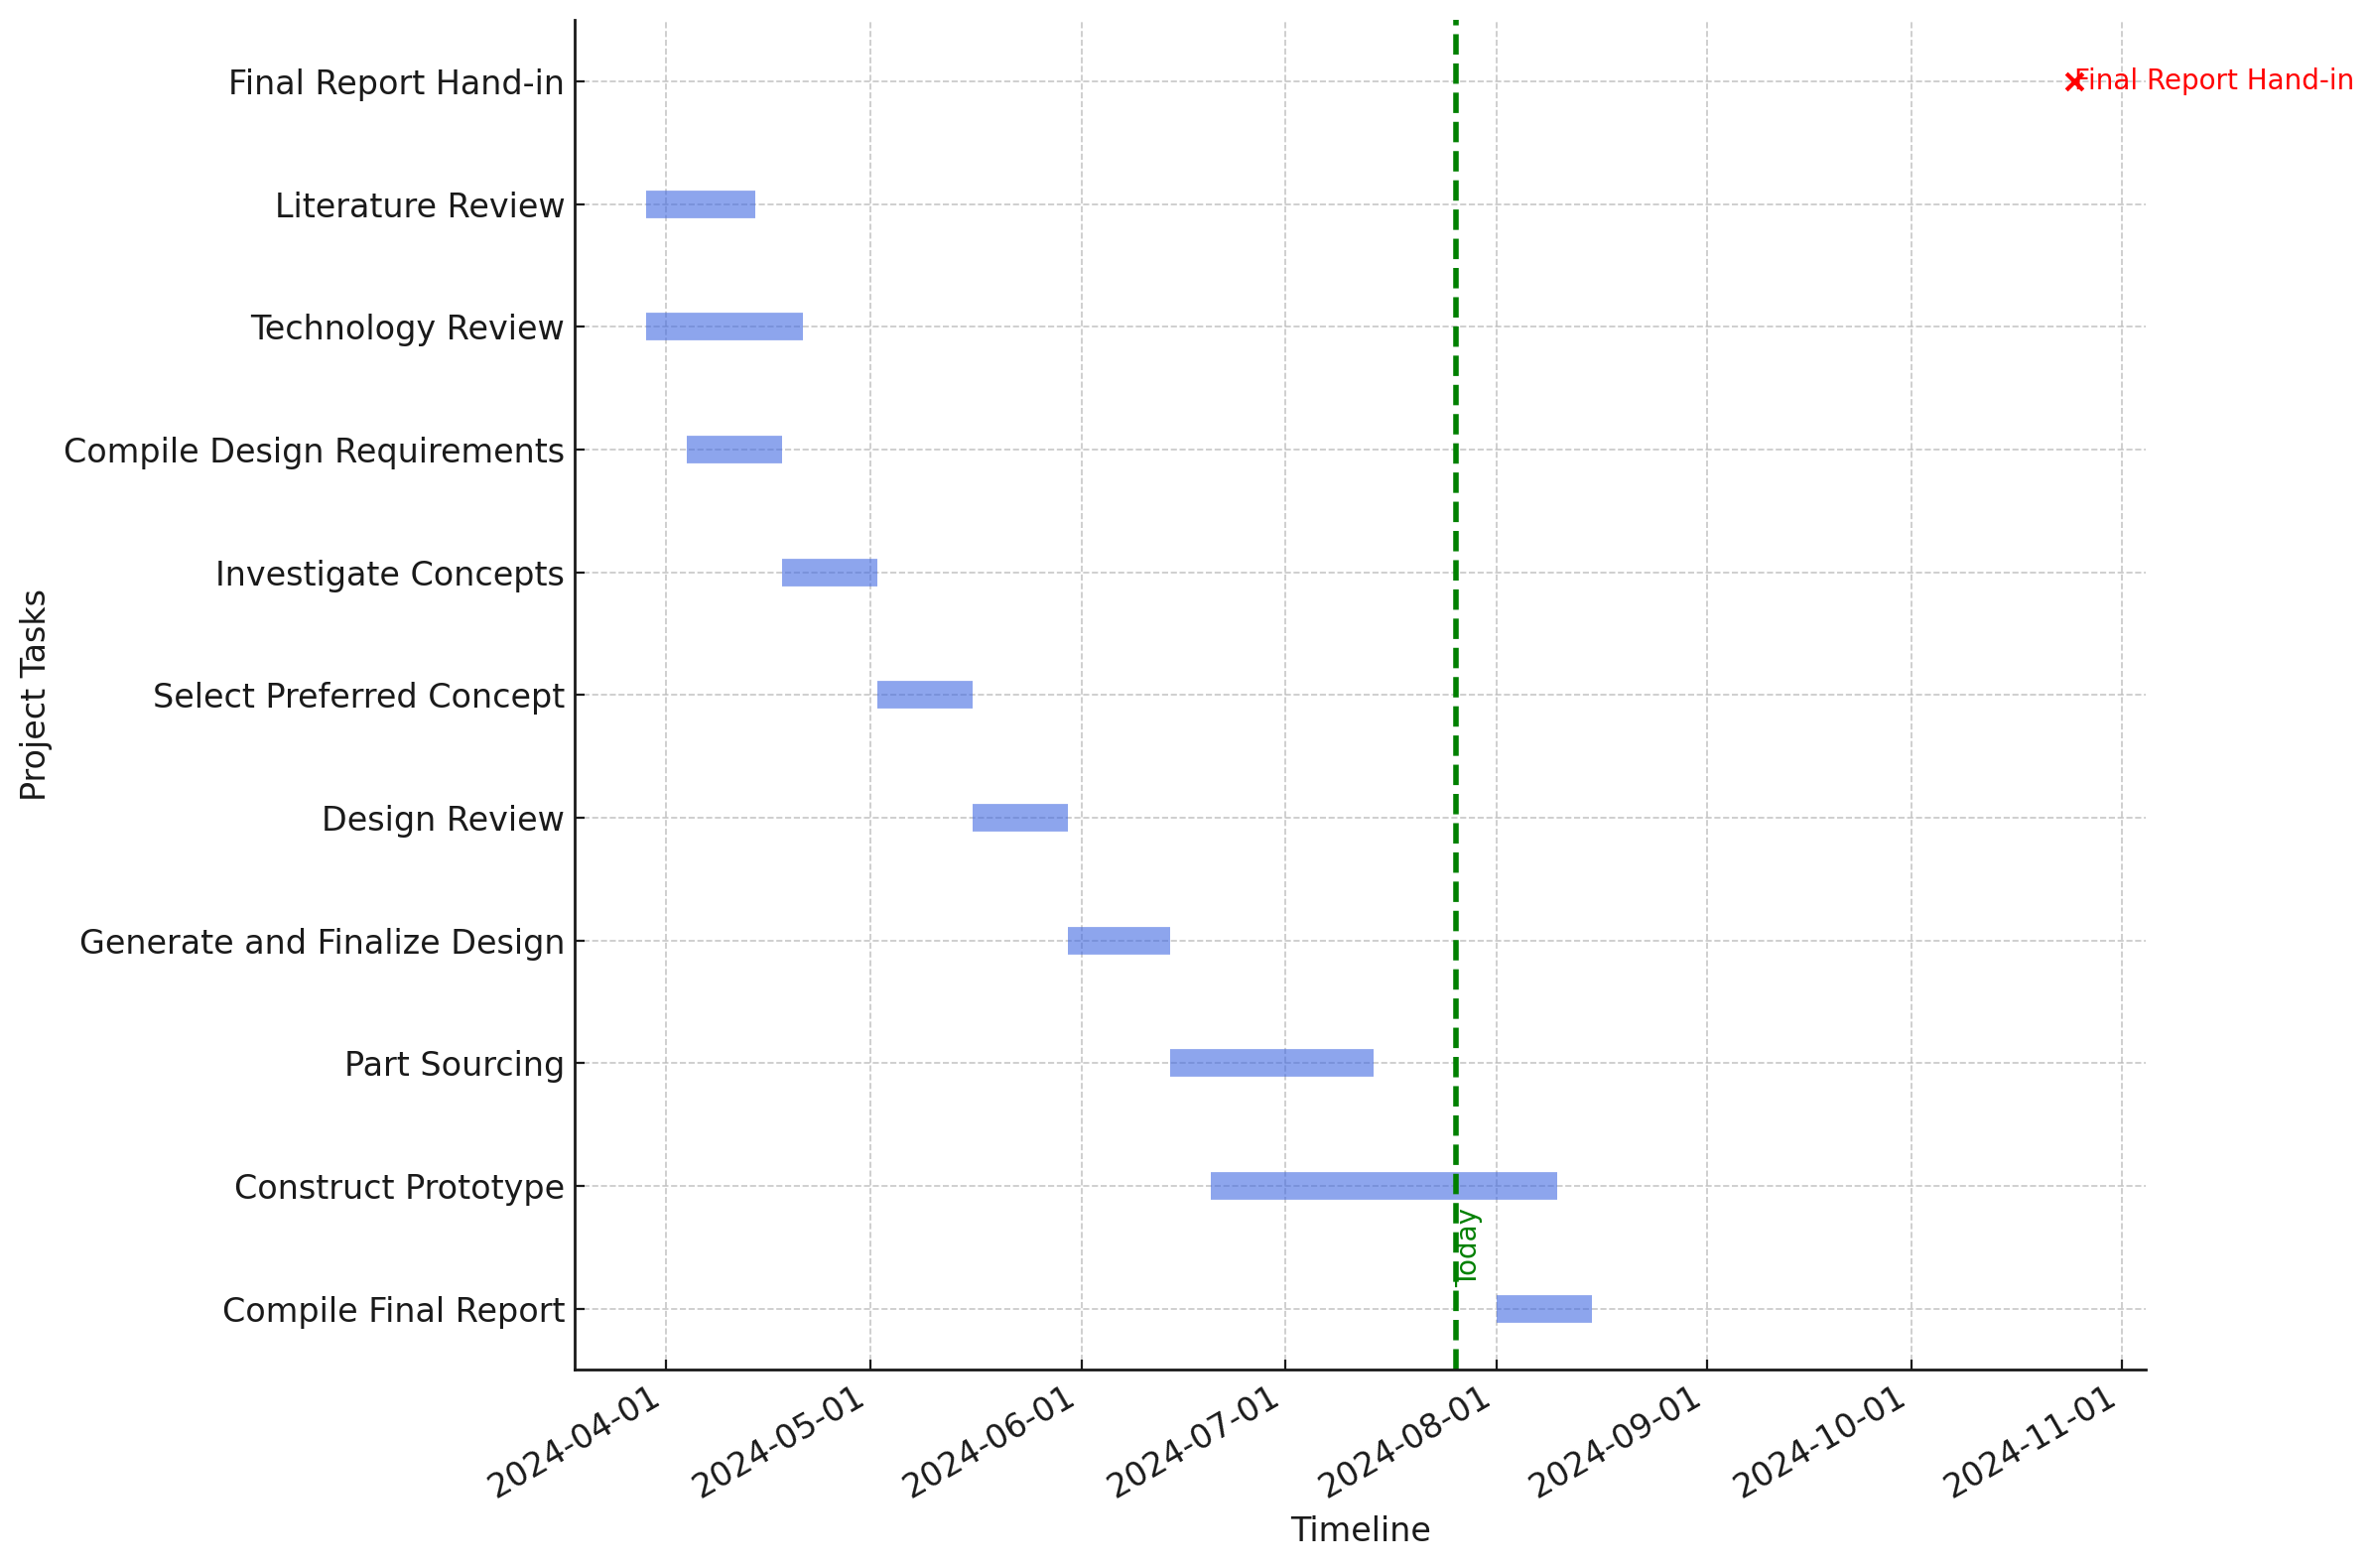
\includegraphics[width=0.75\linewidth]{figs/gantt_progress.png}
    \caption{Initial Gantt Chart with Current Position and Final Report Deadline}
    \label{fig:initial-gantt}
\end{figure}

